\documentclass[sigconf,table]{acmart}
\usepackage{xspace}
\usepackage[caption=false]{subfig}
\usepackage{pifont, enumerate}
\usepackage{footmisc}
\usepackage{balance}
\usepackage[group-separator={,}]{siunitx}
\usepackage{fontspec}
\usepackage{fontawesome5}
\usepackage{booktabs}
\usepackage{hyperref}
\usepackage{footnote}
\usepackage[shortlabels]{enumitem}
\usepackage{booktabs}
\usepackage{csvsimple}
\usepackage{xspace}


\def\nosymbol{\ding{55}}
\def\yessymbol{\ding{51}}
\def\nasymbol{-}

%\newcommand{\revision}[1]{\textcolor{blue}{#1}}
\newcommand{\revision}[1]{#1}


%%%% end data %%%%

\usepackage{amsmath,amssymb}
\usepackage{graphicx}
\usepackage[caption=false]{subfig}
\usepackage[utf8]{inputenc}
\usepackage{url}
\usepackage{xspace}
\usepackage{tikz}
\usepackage{listings}


\usetikzlibrary{arrows,decorations.pathmorphing,backgrounds,fit,positioning,shapes.symbols,chains}

\newcommand{\eg}{\textit{e.g.,}~}
\newcommand{\ie}{\textit{i.e.,}~}
\newcommand{\etc}{\textit{etc.}\xspace}

\newcommand{\mlc}[2][c]{\begin{tabular}[#1]{@{}c@{}}#2\end{tabular}}

\def\faWWWC{\raisebox{-.25em}{
\includegraphics[width=1.75em]{w3c_home_nb-v-bw}}}

\definecolor{tblgray}{gray}{0.9}

%\setlength{\tabcolsep}{.65em}


\copyrightyear{2020} 
\acmYear{2020} 
\setcopyright{iw3c2w3}
\acmConference[WWW '20]{}{}{Taiwan, Taiwan}
%\acmBooktitle{}
%\acmPrice{15.00}
%\acmDOI{10.1145/3243734.3243746}
%\acmISBN{978-1-4503-5693-0/18/10}

\def\thetitle{A Large-Scale Analysis of the use of Integrity Verification Mechanisms for Web Resources}
\def\theshorttitle{Automating the Integrity Verification of Web Downloads for the Masses}

\graphicspath{{figures/}}

\begin{document}

\title[\theshorttitle]{\thetitle}

% alphabetical order (for now...)
%\author{Romain Artru}
% %\orcid{...}
% \affiliation{EPFL\\ Switzerland}
% \email{romain.artru@epfl.ch}
 
\author{Bertil Chapuis} % should be first
 %\orcid{...}
 \affiliation{UNIL -- HEC Lausanne\\ Switzerland}
 \email{bertil.chapuis@unil.ch}

\author{Mauro Cherubini}
 \orcid{0000-0002-1860-6110}
 \affiliation{UNIL -- HEC Lausanne\\ Switzerland}
 \email{mauro.cherubini@unil.ch}
 
\author{Kévin Huguenin}
 \orcid{0000-0001-7147-1828}
 \affiliation{UNIL -- HEC Lausanne\\ Switzerland}
 \email{kevin.huguenin@unil.ch}

\renewcommand{\shortauthors}{Chapuis et al.}

\begin{abstract}

The Subresource Integrity (SRI) recommendation from the W3C ensures that a Webpage can safely integrate subresources hosted on a third-party server.
As Edge Computing and Content Delivery Networks (CDN) get massively adopted, did web developers flocked to the SRI recommendation in order to protect their users?
We conduct a large scale analysis of the CommonCrawl dataset to better understand the adoption of SRI on the Web from its inception in 2016 until 2019.
We highlight the efforts made by different actors to drive the adoption of this recommendation.
We survey web developers to assess their understanding of the security implications of SRI.
Overall, this study presents the most accurate status of the SRI landscape and give hints on what could be done to accelerate the adoption of this important recommendation.
\end{abstract}

\begin{CCSXML}
<ccs2012>
<concept>
<concept_id>10002978.10003014.10003016</concept_id>
<concept_desc>Security and privacy~Web protocol security</concept_desc>
<concept_significance>300</concept_significance>
</concept>
<concept>
<concept_id>10002978.10003029.10011703</concept_id>
<concept_desc>Security and privacy~Usability in security and privacy</concept_desc>
<concept_significance>300</concept_significance>
</concept>
<concept>
<concept_id>10002978.10002979.10002982.10011600</concept_id>
<concept_desc>Security and privacy~Hash functions and message authentication codes</concept_desc>
<concept_significance>100</concept_significance>
</concept>
</ccs2012>
\end{CCSXML}

\ccsdesc[300]{Security and privacy~Web protocol security}
\ccsdesc[100]{Security and privacy~Hash functions and message authentication codes}

\keywords{web security; subresource integrity; checksums}


\def\LatestCCNbURLS{\num{3000000000}\xspace}
\def\LatestCCSize{\num{50}~TB\xspace}
\def\LatestCCDate{2019-08\xspace}
\def\EarliestCCDate{2011-01\xspace}
\def\lastvisited{last visited}
\def\JS{JavaScript\xspace}
\def\BS{beautifulsoup\xspace}
\def\CodeURL{\url{https://link.to.the.code}\xspace}
\def\CCSnapshotN{7\xspace}
\def\CCSnapshotDates{2016-06, 2017-03, 2017-09, 2018-03, 2018-09, 2019-03, and 2019-08\xspace}
\def\CCSnapshotEarliest{2016-06\xspace}
\def\CCSnapshotLatest{2019-08\xspace}

\def\CC{\textit{CC}\xspace}
\def\CCSRI{\textit{CC-SRI}\xspace}
\def\Cisco{\textit{Cisco}}
\def\TopK{\textit{Top1k}}
\def\TopM{\textit{Top1m}}


%%%% begin data %%%%
\def\CCUrlN{\num{2913733422.00}}
\def\CCUrlDistinctN{\num{2884823295.00}}
\def\CCDomainN{\num{49355436.00}}

\def\CCUrlN{\num{2913733422.00}}
\def\CCUrlHttpsN{\num{1395619439.00}}
\def\CCUrlHttpsP{\num{47.90}\%}

\def\CCUrlSriN{\num{74357335.00}}
\def\CCUrlSriP{\num{2.55}\%}

\def\CCOneSriPerWebpageN{\num{36637513.00}}
\def\CCOneSriPerWebpageP{\num{49.27}\%}
\def\CCTwoSriPerWebpageN{\num{25127299.00}}
\def\CCTwoSriPerWebpageP{\num{33.79}\%}
\def\CCOneLinkSriPerWebpageN{\num{30121524.00}}
\def\CCOneLinkSriPerWebpageP{\num{83.06}\%}

\def\CCTreeHttpHttpLocal{\num{1.27}\%}
\def\CCTreeHttpHttpRemote{\num{1.20}\%}
\def\CCTreeHttpHttpsLocal{\num{0.01}\%}
\def\CCTreeHttpHttpsRemote{\num{17.02}\%}
\def\CCTreeHttpsHttpLocal{\num{0.00}\%}
\def\CCTreeHttpsHttpRemote{\num{0.01}\%}
\def\CCTreeHttpsHttpsLocal{\num{5.03}\%}
\def\CCTreeHttpsHttpsRemote{\num{75.46}\%}
\def\CCTreeHttpHttp{\num{2.47}\%}
\def\CCTreeHttpHttps{\num{17.03}\%}
\def\CCTreeHttpsHttp{\num{0.01}\%}
\def\CCTreeHttpsHttps{\num{80.49}\%}
\def\CCTreeHttp{\num{19.50}\%}
\def\CCTreeHttps{\num{80.50}\%}
\def\CCTreeHttpHttpLocalRel{\num{51.35}\%}
\def\CCTreeHttpHttpRemoteRel{\num{48.65}\%}
\def\CCTreeHttpHttpsLocalRel{\num{0.08}\%}
\def\CCTreeHttpHttpsRemoteRel{\num{99.92}\%}
\def\CCTreeHttpsHttpLocalRel{\num{2.08}\%}
\def\CCTreeHttpsHttpRemoteRel{\num{97.92}\%}
\def\CCTreeHttpsHttpsLocalRel{\num{6.25}\%}
\def\CCTreeHttpsHttpsRemoteRel{\num{93.75}\%}
\def\CCTreeHttpHttpRel{\num{12.66}\%}
\def\CCTreeHttpHttpsRel{\num{87.34}\%}
\def\CCTreeHttpsHttpRel{\num{0.02}\%}
\def\CCTreeHttpsHttpsRel{\num{99.98}\%}
\def\CCTreeHttpRel{\num{19.50}\%}
\def\CCTreeHttpsRel{\num{80.50}\%}
\def\CCTreeTotal{\num{100.00}\%}

\def\CCRequireSriForP{\num{0.01}\%}


\maketitle

\sloppy

\section{Introduction} \label{sec:introduction}

The Web is a set of interlinked resources identified by their URL.
A significant portion of these resources consists in HTML webpages that include navigable links and embed subresources, such as scripts, stylesheets, images or videos.
For most of its history, the HTML standard did not enforce the integrity of these subresources embed in web pages, i.e., a change in the subresource will impact the webpage that includes it.
However, the introduction of the recommendation for subresource integrity (SRI) addressed the most pressing aspects of this issue by recommending the use of an integrity verification mechanism for scripts and stylesheets.

Today, due to the advent of Content Delivery Networks (CDN) and Edge Computing, an increasing number of subresources are hosted by third-party providers.
The advantage provided by such platforms are obvious: subresources are hosted at a fraction of the usual cost; subresources are delivered reliably at a low latency.
However, their usage also come at a price: few things prevent a third party service to get hacked or to behave in a malicious way by injecting scripts or defacing stylesheets.

\cite{eden_major_2018}

\subsection{Research Goals}

Given these risks and as discussions take place to extend the SRI standarlarge-scaled to subresources other than scripts and stylesheets, the following questions arise:

\begin{enumerate}
	\item To which extent did web developers and third-party provider adopt the SRI recommendation?
	\item To which extent do web developers understand the threats covered by the SRI recommendation?
	\item What are the forces that drive the adoption of the SRI recommendation since its inception?
	\item What could be done to accelerate and promote the adoption of the SRI recommendation?
\end{enumerate}

\subsection{Contributions and Roadmap}

In this paper, we first disambiguate the threat model associated with the SRI recommendation and highlight its complementarity with HTTPS.
We show that, contrary to a persistent popular belief, SRI is needed even if subresources are served over HTTPS. 

\begin{enumerate}
	\item \textbf{Large-Scale Analysis}
		By using big data processing, we present a large-scale analysis of the use of the SRI recommendation on the Web.
	\item \textbf{Browser Support}
		From the analysis made of the SRI recommendation on the web, we test browser support for SRI according to the corner cases observed on the web. 
	\item \textbf{Web Developer Behavior}
		We survey web developers to asses their understanding of the SRI recommendation and their user experience.
		We verify if their behavior correlates with the observations made in the large-scale analysis.
	\item \textbf{Adoption Incentives}
		 We discuss the driving forces behind the adoption of SRI and give hints on what could foster its larger adoption in the future.
\end{enumerate}



\section{What is SRI?}

\subsection{Overview or the Recommendation}

Subresource Integrity (SRI) let browsers verify that the subresources of a webpage are fetched without manipulation.
Whereas this mechanism can be used with any subresource, the intent of the recommendation is to assert the integrity of resources served by third party services, such as CDNs.
This security feature allows the web developer to include a cryptographic checksum in the HTML that the downloaded subresource must match in order to be included.
As of June 2019, SRI is fully supported by Chrome, Firefox, Opera and Safari, and partially supported by Edge.

\begin{lstlisting}[language=HTML, basicstyle=\small]
<script src="example.js" 
	integrity="sha256-TWupyv..." 
	crossorigin="anonymous" />
\end{lstlisting}

Content Security Policy (CSP) let web developers mitigate certain kind of attacks, such as Cross Site Scripting (XSS), by specifying directives that delimitate the trust given to third party services.
In the context of SRI, CSP directives can be used to mandate the web developper to include an integrity attribute for certain subresources. 
For instance, this can be achieved by specifying the following meta element in the head of the web page: 

\begin{lstlisting}[language=HTML, basicstyle=\small]
<meta http-equiv="Content-Security-Policy" 
      content="require-sri-for script;">
\end{lstlisting}

Or by specifying the following HTTP header in the configuration of the web server:

\begin{lstlisting}[basicstyle=\small]
Content-Security-Policy: require-sri-for script;
\end{lstlisting}

The latter mechanism has the advantage of enabling a separation of concerns between the web developer and the system administrator, who is usually more concerned by security issues.
Managing SRI at the level of the configuration of the server enables the system administrator to force the adoption of the recommendation at a higher level.
Unfortunately, due to its poor adoption, web browsers slowly abandon this directive.

Interestingly, given an integrity attribute, the SRI recommendation allows to specify multiple checksums (See SRI section 3.6), each of which is prefixed by the name of the hash function used to generate it followed by a dash (e.g., sha256-).
This allows the browsers to pick the strongest hash algorithms, but also to specify several hash values for the same URL, which might be useful during a rolling upgrade.
 

\subsection{Threat Model}

\begin{figure}
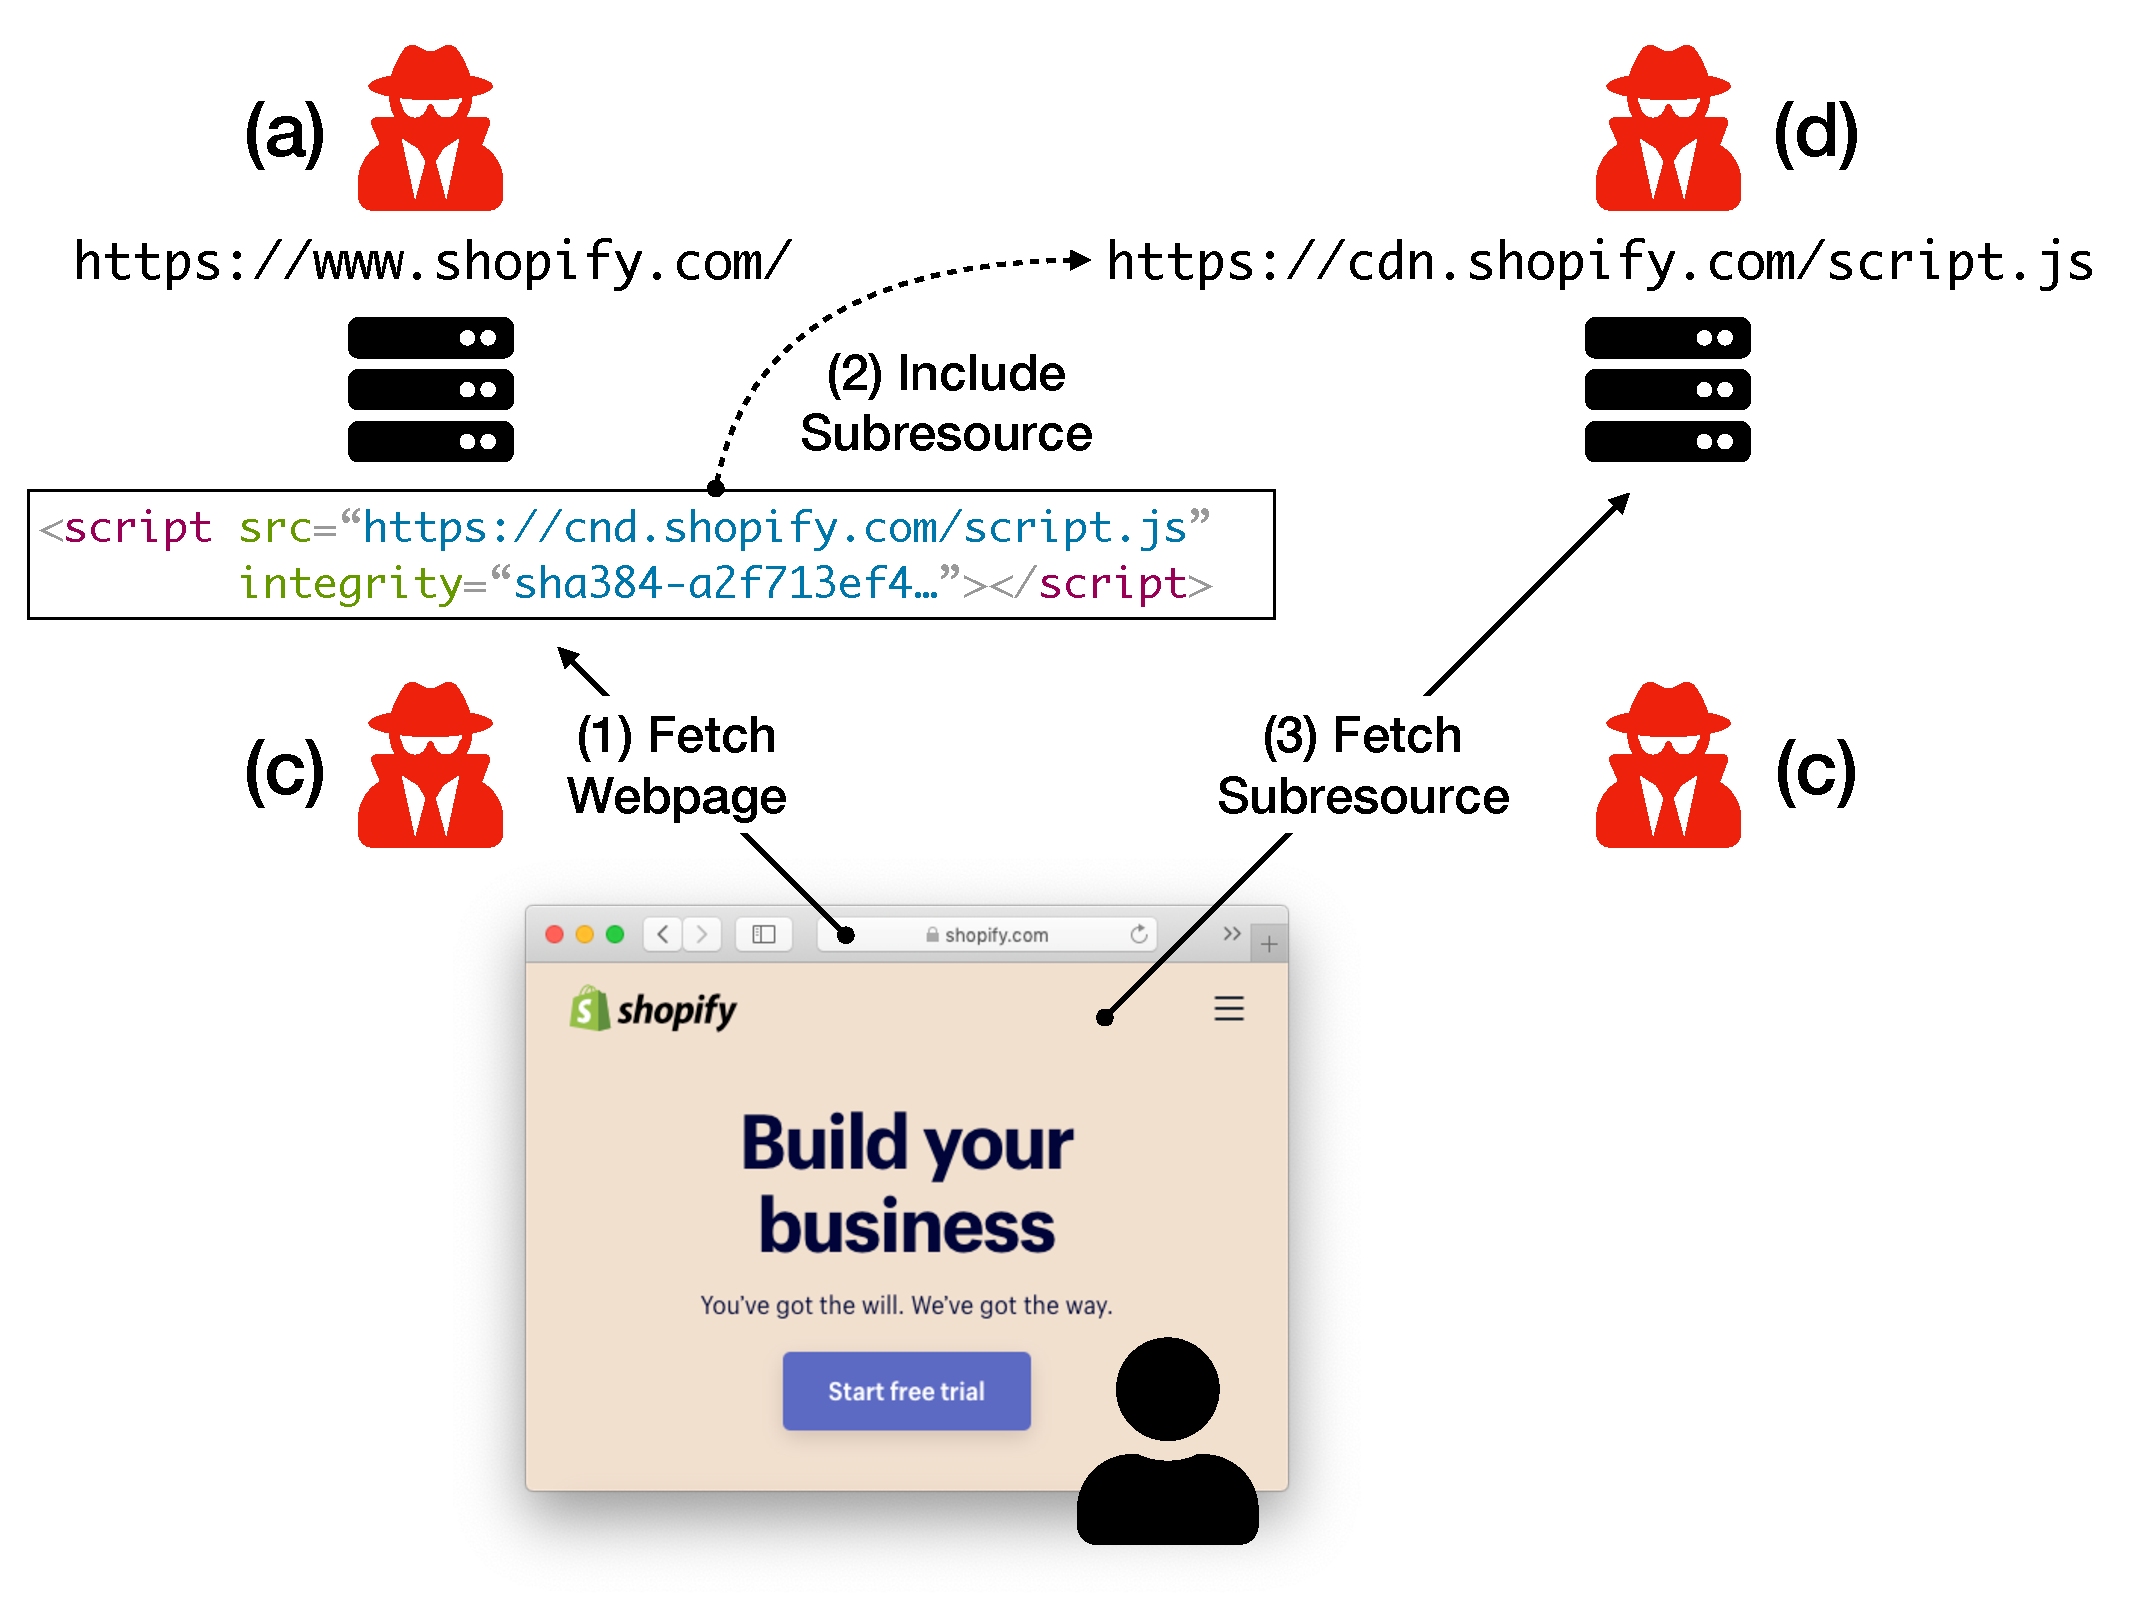
\includegraphics[width=\columnwidth]{figures/model}
	\caption{Simplified threat model for HTTPS and SRI}
	\label{fig:model}
\end{figure}


The design goal of the SRI recommendation is: "to define a mechanism by which user agents may verify that a fetched resource has been delivered without unexpected manipulation".\footnote{\url{https://www.w3.org/TR/SRI/}}
The HTTPS specification share a common objective with SRI: "SSL, and its successor TLS were designed to provide channel-oriented security".\footnote{\url{https://tools.ietf.org/html/rfc2818}}
Despite the fact that the two standards seem to overlap, HTTPS provides channel integrity by authenticating the server, whereas SRI provides subresource integrity by authenticating the content.

Figure~\ref{fig:model} illustrates a simplified threat model for HTTPS and SRI that helps understanding the threats covered by the specification and the recommendation.
We consider an HTML webpage delivered by a server managed by a web developer. 
The webpage includes a script element that references a subresource (e.g. a JavaScript program or a CSS stylesheet) hosted on another server, typically managed by a third-party.
In order to enable browsers to check the authenticity of the subresource, the webpage specifies an integrity attribute for the subresource.
We consider four possible adversaries who could tamper with the webpage:

\begin{enumerate}[(a)]
\item 
	The attacker gains access to the server managed by the web developer and tempers with the webpage. 
	If this server gets compromised, neither HTTPS nor SRI help at protecting the users.
	Therefore, we assume that the server managed by the web developer is secure and trusted.
\item 
	The attacker tempers with the communication channel between the server hosted by the web developer and the users.
	A web page served over HTTP is vulnerable to such attack.
	Therefore, we assume that HTTPS is trustworthy in preventing their occurrences.
\item 
	The attacker tampers with the communication channel between the third-party server that hosts the subresource and the users.
	If the subresource is served over HTTP, SRI can prevent the execution of a compromised subresource by authenticating its content.
	However, HTTPS should be preferred as it provides authenticity at the level of the channel.
\item 
	The attacker gains access to the third-party server and tampers with the subresource.
	If the third-party server gets compromised, HTTPS is of no help, i.e., nothing prevent the attacker from modifying the subresource.
	SRI precisely addresses this issue: if the hash of the subresource does not match the integrity attribute, the browser prevents its inclusion and execution.

\end{enumerate}

As highlighted here, the SRI recommendation covers a unique spot at the level of the third-party server that hosts subresources; a scenario which is far from being marginal in today's decentralized context.
For instance, a CDN typically rely on a network of geographically distributed servers, each of which can get individually compromised, affecting a subset of the users.
In fact, in the context of a CND, having the same domain for all resources does not mean that they are located on the same serve, hence the importance of content authenticity.
Therefore, as web developers increasingly rely on CDNs to deliver their content, a mechanism that enables them to guarantee the integrity of subresources is necessary to mitigate this kind of attacks and the widespread adoption of SRI becomes critical. 


\subsection{Developers' Behavior}

When it comes to the adoption of SRI by web developers, the development practices they adopt are of great importance.
In this Section, we describe the most popular web application architectures, we highlight the build tools associated with them, and give hints on how these tools can influence the behavior adopted by web developers.

\subsubsection{Multi Page Application (MPA)}

Traditionally, each action performed by the user on an HTML webpage (clicking on a link, submitting a form) generates an HTTP request.
A web server typically respond to requests with new HTML webpages, which are displayed in the browser.
That is the multi page application (MPA) architecture.
Web developers usually modify the server side templates to include JavaScript and CSS libraries (such jQuery or Bootstrap) in the head of the HTML.

\subsubsection{Single Page Application (SPA)}

More recently, the single page application (SPA) paradigm started to gain in popularity with frameworks such as Angular, ReactJS, or VueJS.
These applications load a single HTML webpage and, later on, dynamically update their content.
To do so, these application bypass the traditional way of loading webpages by URLs.
The content displayed in the application is transmitted with a micro-format, such as JSON, and its rendering occurs in the browser instead of on the server.
The root page of an SPA is often managed with a build tool that includes the necessary dependencies in the head of the HTML.
Web developers usually modify a configuration file, which is then used to inject development or production versions of the dependencies.


\section{Large-Scale Analysis} \label{sec:analysis}

In this section, we report on the analysis of the use of SRI on the Web. We describe our datasets and our methodology and we present our results.

\subsection{Data sources}

\subsubsection{Common Crawl (\CC)}

% sampling/crawling method?
The Common Crawl (\CC) dataset is a collection of snapshots of the Web.\footnote{\url{http://commoncrawl.org/}}
It contains one snapshot per month since \EarliestCCDate. Each snapshot comes in three flavors: the WARC format which contains the raw data of the webpages (HTTP headers and HTML content but not the content of the subresources), the WAT format which contains the metadata of the webpages (HTTP headers and the hyperlinks contained in the webpage) and the WET format which contains the plaintext extracted from the webpages.
The latest snapshot of Common Crawl (\LatestCCDate) weighs \LatestCCSize and contains \LatestCCNbURLS~URLs.\footnote{More statistics are available at: \url{https://commoncrawl.github.io/cc-crawl-statistics}, \lastvisited: Sep. 2019.}
Each snapshot (in each of the format) is divided into multiple archives so as as to enable parallel and distributed processing of the dataset. The \CC dataset is publicly available on Amazon S3, where it can be processed and analyzed using Amazon EMR using frameworks such as Hadoop and Spark.
In this paper, we rely on the \CC dataset to analyze the prevalence of SRI on the Web and its evolution over time.

% replace with Igor's
\subsubsection{Cisco Umbrella 1 Million (\Cisco)}

The Cisco Umbrella (\Cisco) dataset is a ranking of the top 1 million most popular domains names.\footnote{\url{https://umbrella.cisco.com/blog/2016/12/14/cisco-umbrella-1-million/}}
The algorithm used to generate this dataset uses DNS queries (100 Billion requests/days) and client IPs (65 million unique users) to measure the aggregated popularity of a domain name.
As the Cisco Umbrella network is global (165 countries), it is representative of the overall traffic on the Web.
Despite the fact that this dataset is not confined to HTTP traffic, we prefer it to the popular Alexa 1 Million dataset, which is not available in open access anymore.\footnote{https://www.alexa.com/topsites}
We sometimes use the top 1 thousand (\TopK) and top 1 million (\TopM) domains extracted from the \Cisco\ dataset to bound our metrics to the most visited part of the Internet.


\subsection{Methodology}
% add version everywhere


In order to study the use of SRI on the Web, we need to extract the subresources contained in webpages and therefore to parse their HTML content.
Parsing the content all the webpages contained in a snapshot of \CC is very time consuming, and hence expensive.
As our analysis focuses on the use of SRI, we rely on a simple filter to detect webpages containing subresources with an integrity attribute.
More specifically, we keep only the webpages that contain the string ``integrity=''.
Note that this filtering is done on the \emph{static} (i.e., returned by the server, without any client-side manipulation such as \JS execution) \emph{raw} (i.e., in the binary format, that is before decoding) content of the webpages; this can lead to false negatives (i.e., filtering out webpages that do contain subresources with an integrity attribute).
We further detect the encoding of the webpages and parse them by using the \texttt{\BS} library (vXX) with the \texttt{lxml} parser.
This enables us to extract the subresources of the webpages (and their attributes) and to filter out the webpages that do \emph{not} contain any subresource with an integrity attribute (that have not been filtered out because they do contain the string ``ìntegrity='' but somewhere else in the webpage).
This constitutes the set of webpages on which we conduct our analysis, namely the ``webpages that contain at least one SRI'' set (\CCSRI).
For each webpage in the \CCSRI dataset, we extract its URL, content security policy (CSP) (from the header),  and all its \texttt{link} and \texttt{script} elements/subresources.

In order to study not only the current use of SRI but also its evolution, in our analysis, we process a total of \CCSnapshotN \CC snapshots from \CCSnapshotEarliest to \CCSnapshotLatest (more specifically \CCSnapshotDates).
Note that the SRI specification was issued by the W3C in late June 2016.

%2016-18: n/a
%2017-09: 55.88TB
%2017-34: 65.14TB  
%2018-09: 71.96TB 
%2018-34: 67.79TB 
%2019-09: 59.86TB

%The resulting parquet file follows the following structure:
%
%\begin{enumerate}
%	\item \textit{warc} The id of the warc file containing the webpage.
%	\item \textit{url} The url of the webpage.
%	\item \textit{csp} The content-security-policy header of the webpage.
%	\item \textit{subresources (element, target, integrity, crossorigin)} The list of subresources with or without SRI included in the webpage.
%	\item \textit{error} A flag indicating if an error occured while parsing the webpage.
%\end{enumerate}

%The subset (parquet files) for February 2019 weight approximately 100GB and covers \CCUrlSriP\ of webpages present in the \CC dataset.

%\subsubsection{Post-processing}

%As the resulting parquet files are not "big" anymore (598GB), we repatriated them on a local server to perform our analysis (post-processing).
%We used Python and Spark SQL to query the parquet files.
%The resulting Spark data frames are converted into Pandas data frames in order to be plotted or exported.




% 01: What is the number of pages by protocol?
\subsection{Results}

\subsubsection{HTTPS Adoption}

As the HTTPS protocol provides channel integrity, we measured its adoption in the \CC dataset.
The \CC dataset stores the complete URLs of the webpages and we parsed them to extract the protocol in use.
In addition, we filtered the \CC dataset with the \TopK\ and \TopM\ datasets understand how the most visited part of the Web are evolving in terms of protocol.

Figure~\ref{fig:01} displays the evolution of the percentage of webpages served over HTTPS for the \CC dataset and its subsets (\TopM, \TopK).
As of writing, almost half of the websites (\CCUrlHttpsP) and most of the websites in \TopK and \TopM switched from HTTP to HTTPS and the adoption seems to be reaching a plateau.
Interestingly, the adoption of HTTPS measured for the \TopK\ domains in 2016 is close from the adoption measured in Chrome at the same period by Felt et al~\ref{}, which highlights the incredible progress made by popular websites in adopting HTTPS.
Massive and fruitful efforts have been leveraged to accelerate the adoption of HTTPS.
The release of let's encrypt (2016-04-12) and of the ACME protocol v1 (2016-04-12) and v2 (2018-03-13), which automates the deployment of public key infrastructure, played a major role in the adoption for HTTPS.
The introduction of security warnings in Firefox (2017-03-07), Chrome (2018-07-24) and Safari (2018-07-09) for webpages served over HTTP have also been an effective incentive, in the sense that end-users complains about security warning affects web developers directly.
Internet Explorer and Microsoft Edge did not yet introduced security warnings for HTTP webpages.
However, the adoption of the Chromium platform by Microsoft Edge suggests that very soon all major browsers will visually encourage the adoption of HTTPS.


% Warnings:
% Firefox 52 (2017-03-07)
% Chrome 68 (2018-07-24)
% Let's Encrypt and ACME v1 (2016-04-12)
% ACME v2 (2018-03-13)
% Safari 11.1.2 (2018-07-09)
% Edge (no visual warning)

\begin{figure}[h]
	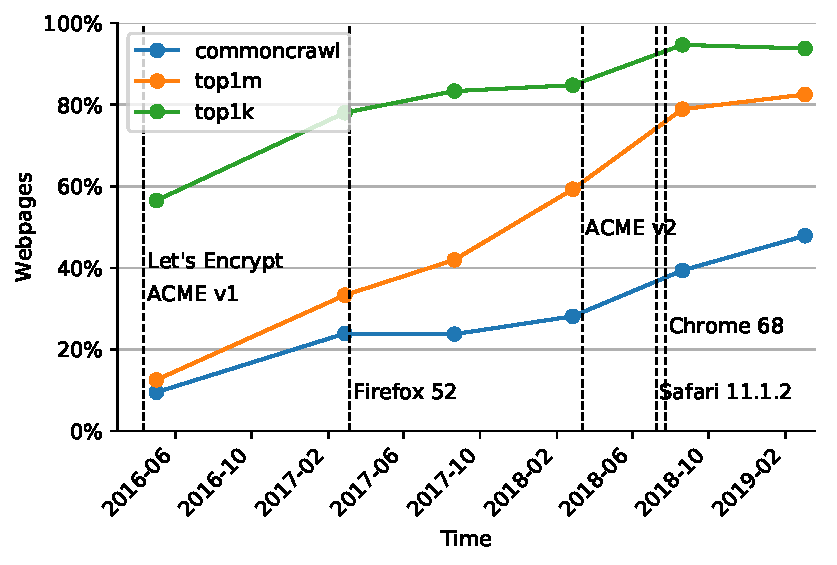
\includegraphics[width=\columnwidth]{../../notebooks/01_pages_per_protocol}
	\caption{Evolution of the percentage of webpages served over HTTPS}
	\label{fig:01}
\end{figure}

% 02: What is the number of pages that include at least one SRI?

\subsubsection{SRI Adoption}

The release of the SRI recommendation in June 2016 officially enabled its wide spread adoption by web developers.
To measure the extent of this adoption, we study the use of the integrity attribute across all the versions of the \CCSRI dataset.
To do so, we count the webpages that include at least one subresource that specifies the integrity attribute for \textit{script} element, the \textit{link} elements and the combination of the two (\textit{any tag}).
Additionally, we filter the \CC dataset with the \TopK\ and \TopM\ datasets to measure the adoption of the integrity attribute in the most visited parts of the Web.

Figure~\ref{fig:02} depicts the evolution of the percentage of webpages containing at least one element that specifies the integrity attribute over time.
overall, the adoption of SRI is slowing down; this slow down particularly affects the \textit{script} element and spare the \textit{link} element.
This might be explained by the increasing popularity of the SPA architecture to the detriment of the MPA architecture.
Whereas the aging MPA architecture promoted the inclusion of libraries, such as jQuery, by copy pasting snippets in the head of the webpage, the SPA architecture often rely on build tools that inject scripts in the webpage but lack support for SRI.
In this context, the use of the integrity does not affect the \textit{link} element, which might be due to the growing popularity of the \textit{Font Awesome} library, which still seems to be mostly included in webpages by copy pasting a snippet.
Interestingly, a minor fraction of the webpages started including the integrity attribute before the release of the recommendation in June 2016.
Most notably, the popular bootstrap framework started to provide code snippets containing the integrity attribute since October 2015, which highlights the living nature of the HTML standard.
Finally, it can be observed that the adoption of the SRI recommendation by the \TopK and \TopM websites started late but accelerates very fast.
This might be due to the fact that popular websites operated their own servers until recently and started to rely on third-party CNDs once their advantages became obvious.
Today, as popular websites increasingly rely on CDNs and third party services, justified security concerns probably drive this adoption.

\begin{figure}[h]
	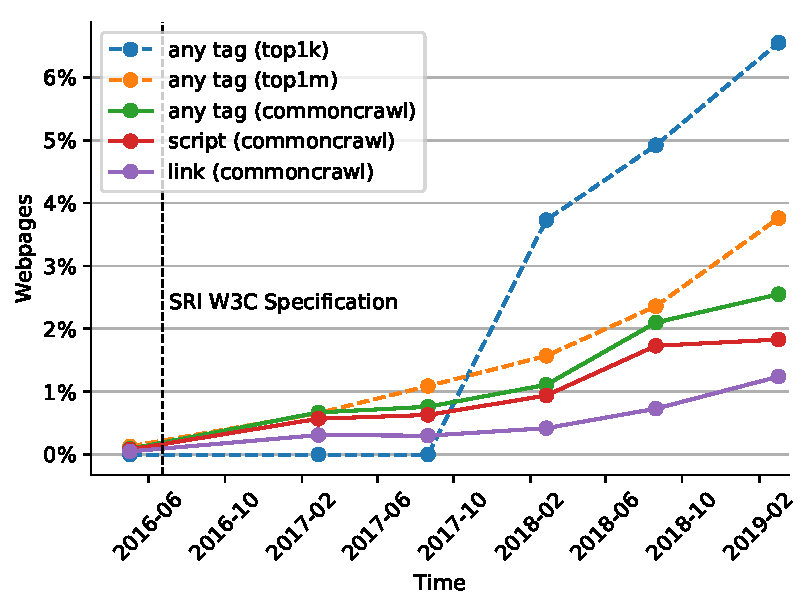
\includegraphics[width=\columnwidth]{../../notebooks/02_pages_with_sri}
	\caption{Evolution of the percentage of webpages containing one or more tag (script or link) that specifies the integrity attribute}
	\label{fig:02}
\end{figure}

% TODO: August Crawl

% SRI W3C recommendation (2016-06-23)

\subsubsection{Subresources per Webpage}

A webpage can contains subresources that specify the integrity attribute along side subresources that do not specify it.
We queried the \CCSRI dataset to obtain the mean number of subresources per webpages (with and without integrity attribute) and the associated standard deviation at different point in time.

Figure~\ref{fig:03-evolution} displays the mean and standard deviations for subresources with and without the integrity attribute.
The mean number of subresource with the integrity attribute per webpage is low and revolve around two.
The large discrepancy between the mean number of subresources and the mean number of subresource without the integrity attribute suggests that web developers copy paste one or two code snippets that specify the integrity attribute in the head of their webpage.
In addition, it seems to indicate that the automatically injection of SRI in webpages by built tools did not yet gained traction.
In conclusion, the fact that the mean and standard deviation remained stable over time suggests that a shift in behavior (similar to what occurred for HTTPS) that would significantly improve the adoption of SRI did not occur yet.

\begin{figure}[h]
	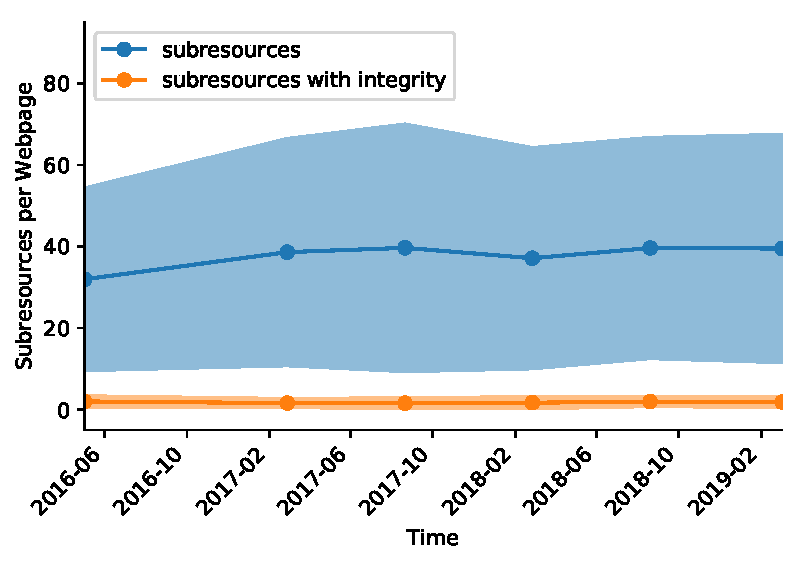
\includegraphics[width=\columnwidth]{../../notebooks/03_pages_per_sri_evolution}
	\caption{Mean and standard deviation of the number of subresources per webpage, among webpages that contain at least one SRI (\CCUrlSriP)}
	\label{fig:03-evolution}
\end{figure}

% 03: What is the number of pages per number of number SRI?

\subsubsection{SRI per Webpage}

The integrity attribute is supported by the \textit{script} and \textit{link} elements, which are used to load external subresources in webpages, such as script or stylesheets.
We queried the \CCSnapshotLatest snapshot of the \CCSRI dataset and counted the number of occurrence of the integrity attribute associated with these elements.
 
Figure~\ref{fig:03} depicts the PDF/CDF for the integrity attribute in the \CCSnapshotLatest snapshot of the \CCSRI dataset.
It can be observed that, regardless of the element (\textit{any tag}), \CCOneSriPerWebpageP of webpages contain one integrity attribute and \CCTwoSriPerWebpageP of webpages contain two integrity attribute.
The same observation holds when looking at the \textit{script} element, i.e., web developers regularly include more than one element that specifies the integrity attribute.
When it comes to \textit{link} elements, the web developer's behaviour is slightly different, as \CCOneLinkSriPerWebpageP\ of them specify the integrity attribute only once.
Overall, the fact that the number of elements that specify the integrity attribute is very low suggests a copy-paste behavior from Web developers, who simply integrate the snippets provided by popular javascript and css libraries, such as JQuery and Bootstrap.

\begin{figure}[h]
	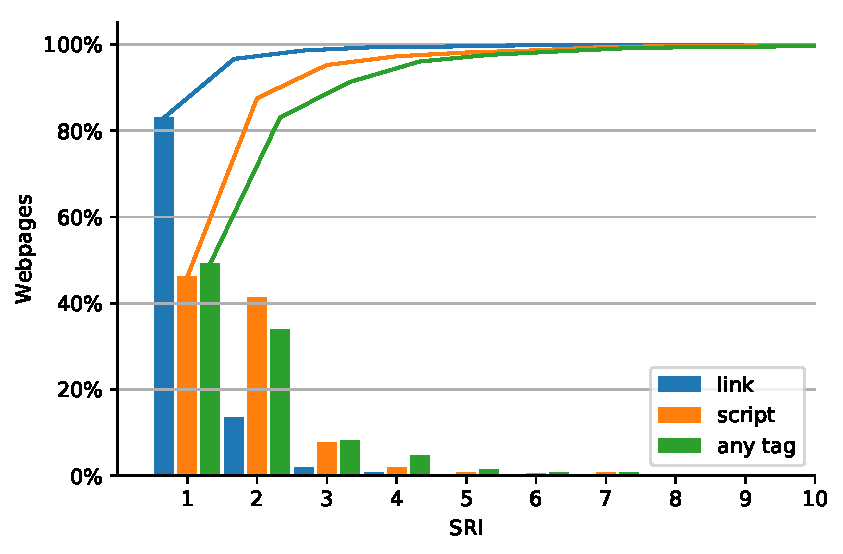
\includegraphics[width=\columnwidth]{../../notebooks/03_sri_per_page}
	\caption{PDF/CDF of the number of SRI per webpages, among webpages that contain at least one SRI (\CCUrlSriP)}
	\label{fig:03}
\end{figure}







% 04: What is the number of SRI per hash algorithm?
\subsubsection{SRI Hash algorithms}
%\paragraph{Background}
SRI relies on the SHA2 hash algorithms for producing the digests included in integrity attributes; it allows for different digest sizes, essentially 256, 384 and 512 bits.
The size of the digest used is specified at the beginning of the integrity attribute, followed by the base-64 encoded digest.
SRI allows multiple (space-separated) digests in an integrity attribute; in this case, the subresource is loaded by the user agent if \emph{at least} one of the digests matches that of the downloaded subresource or if the integrity attribute is malformed.

More specifically, an SRI integrity attribute follows the CSP Level 2 rules below. For instance, ``\texttt{sha256-ZdAL...smUg= sha384-Cq5f...h0kN}'' is a valid integrity attribute with two digests of size 256 and 384 respectively:
%KH: don't get the format; also, it doesn't account for multiple digests. IS it really needed?
\begin{lstlisting}[basicstyle=\footnotesize]
base64-value = 1*( ALPHA / DIGIT / "+" / "/" )*2( "=" )
hash-value   = base64-value
hash-algo    = "sha256" / "sha384" / "sha512"
hash-source  = hash-algo "-" hash-value 
\end{lstlisting}

%\paragraph{Methodology}
We study the sizes of the digests and the number of digests used in integrity attributes (for \texttt{link} and \texttt{scripts} elements) across the latest version of the \CCSRI dataset (\CCSnapshotLatest). To do so, we analyze all the integrity attributes in the dataset; for each integrity attribute, we parse it according to the rules specified above. More specifically, we re-implemented the parsing and validation performed in Firefox v?. If the parsing or the validation fails, the attribute is considered malformed (and labeled as such). In our analysis, we distinguish malformed and empty attributes. Note that subresources with an empty integrity attribute are loaded by user agents. For the well-formed attribute, we extract the digest size(s) and label the attribute accordingly. When an integrity attribute contains multiple digests, e.g., SHA-256 and SHA-384, we label it with the different sizes (e.g., ``SHA-256+SHA-384''): we use different labels for the different combinations of digest sizes. 

%\paragraph{
Figure~\ref{fig:04} depicts the distribution of the digest sizes across all the \texttt{link} and \texttt{scripts} elements with an integrity attribute in the dataset. It can be observed that most integrity attributes contain only one digest, and that the most popular lengths are SHA-384 and SHA-256 (in that order).
Only a few percents of the integrity attributes contain more than one digest.
We did not observe any integrity attribute with multiple digests of the same size (e.g., two SHA-256 digests), which is surprising. % KH: are we sure that this is not because of our methodology? Did you look at all the sizes or just the list of unique sizes (without duplicates)?
Indeed, using several digests enables webmasters to handle multiple version of a script by including the digests of all the supported versions (if the version of the script is not specified in the URL).
In such a case, however, there is no particular reason to use different digest size.
A possible explanation is that some webmasters misunderstood how the case of multiple digests is handled by user agents: They might have thought that having more than one digest increases the security of the integrity verification; it is actually the opposite as the subresource is loaded as soon as one of the digests matches that of the downloaded subresource.
%KH: please check the argument above
A very small (yet not negligible) proportion of the attributes are left empty. This is the case of the subresources on the Apple iTunes website. For the malformed integrity attributes, we manually investigate them; the causes include: missing hash algorithms (e.g., ``Cq5f...''), unsupported hash algorithms (i.e., ``md5''), mistyped hash algorithms (e.g., ``ha256''), and injection through client-side template (e.g. ``\{\{CHECKSUM\}\}''). Note that in this last example, the use case might be eventually be valid if the value of the attribute is (correct and ) indeed inserted at the client side before the verification is made by the user agent.

\begin{figure}[h]
	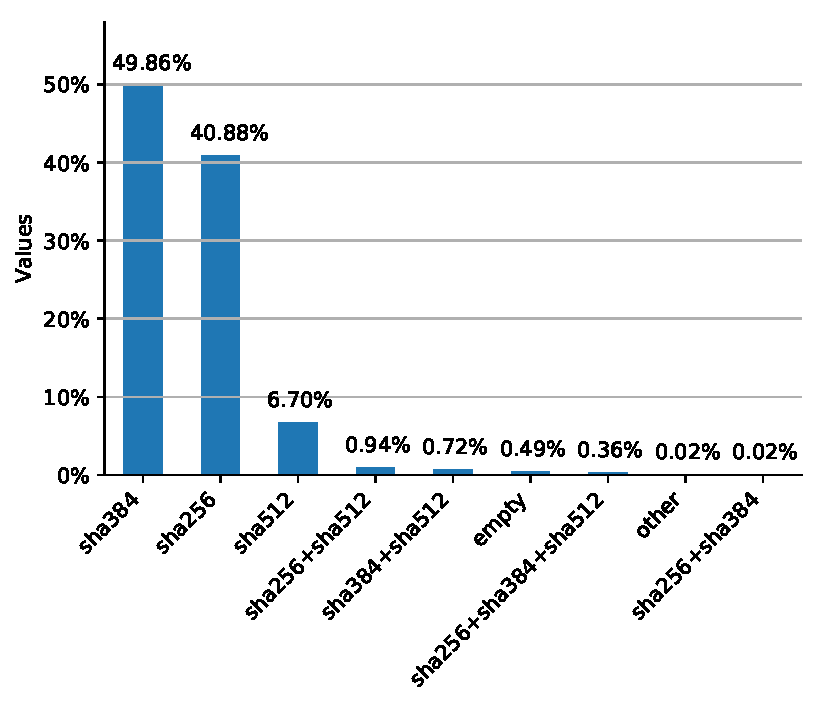
\includegraphics[width=\columnwidth]{../../notebooks/04_sri_per_algorithm}
	\caption{Distribution of the hash algorithms used to compute the checksums included in the value of the integrity attribute (the integrity attribute can specify more than one checksum).}
	\label{fig:04}
\end{figure}

\subsubsection{Distribution of SRI per host and target protocol}

The protocol used by a webpage does not necessarily match the protocol of its subresources.
For instance, a webpage served over can include an HTTPS subresource, whereas the reverse is not permitted by modern Web browsers for security reasons.
In this context, the \textit{host} protocol refers to the protocol used to serve the webpage that include the subresource.
The \textit{target} protocol refers to the unresolved protocol specified in the \textit{src} or \textit{href} attributes of the subresource included in the webpage.
In practice, this \textit{target} protocol can be specified explicitly (http://, https://), or implicitly, i.e., the protocol is inherited when the path is relative (.) or absolute (/) and when the URL use protocol inheritance (//).


Figure~\ref{fig:06} depicts the distribution of subresources that specify the integrity attribute by \textit{host} and \textit{target} protocol.
We observe that most of the \textit{targets} fall into the absolute URL categories (http://, https:// and //).
As the integrity attribute does not make a lot of sense in the context of relative URLs, we can assert that, in this regard, the SRI recommendation is well used and understood.
Interestingly, the extensive use of protocol inheritance for \textit{targets} (//), which allows to gracefully upgrade a website from HTTP to HTTPS, is syntactic sugar, as it is mostly used on webpages served over HTTPS.
	
\begin{figure}[h]
	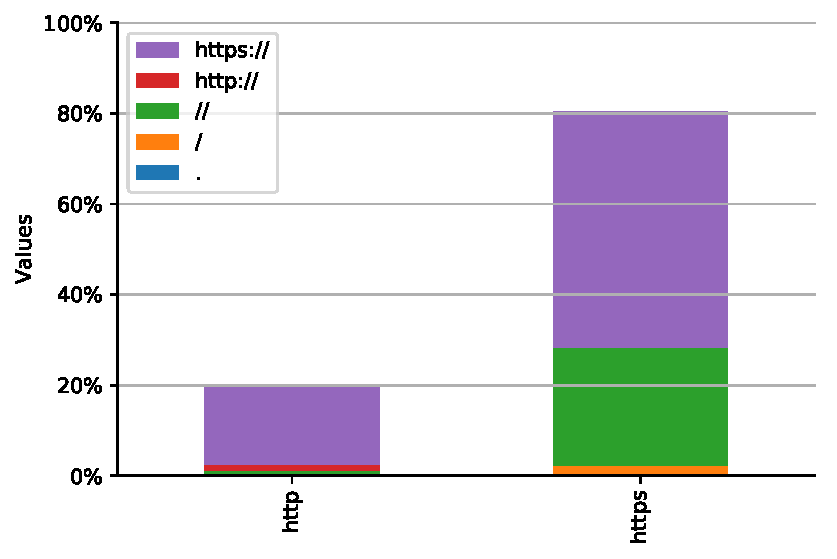
\includegraphics[width=\columnwidth]{../../notebooks/06_sri_per_host_and_target_protocol}
	\caption{Distribution of SRI per host and target protocol}
	\label{fig:06}
\end{figure}


\subsubsection{Categorization of SRI per host protocol, target protocol and locality}

The domain used by a webpage does not necessarily match the domain of its subresource.
Given the fact that webpages served on the same domain are not necessarily served by the same server, the integrity attribute is of interest even if the domains are the same.
However, when subresources are hosted on a CDN, it is common to observe a  such a domain mismatch.
Therefore, we queried the \CCSnapshotLatest snapshot of the \CCSRI dataset to categorize the subresources that specify the integrity attribute per \textit{host} protocol, \textit{target} protocol and \textit{locality} .
Here, the \textit{host} refers to the domain and protocol of the webpage, the \textit{target} refers to the domain and resolved protocol of the subresource, and \textit{locality} tells if the domain and protocol of the \textit{host} is the same as the domain and protocol of the \textit{target} (local or remote).

The tree depicted in Figure~\ref{fig:07} breaks down our results according to the aforementioned criterion.
The first level of the tree shows that the majority of websites using SRI (\num{80.50}\%) already adopted HTTPS.
Given the fact that \num{17.03}\% of the subresources having an HTTP \textit{host} have an HTTPS  \textit{target}, the second level shows that overall the vast majority of subresources are already served over HTTPS (\num{97.53}\%).
The third level shows that \num{80.49}\% of the subresources specifying the integrity attribute are protected against all the attacks mentioned in the Threat model.
However, \num{17.02}\% of the subresources are still exposed to tampering at the level of the communication channel (see (b) and (d) in Figure~\ref{fig:model})
The third level highlight that misuses of the HTTPS specification, such as downgrade of the protocol from HTTPS to HTTP, are very rare (\num{0.01}\%).
In case of downgrade, the user is not exposed to a security risk. However, his experience is degraded as the subresource is not included in the webpage by the browsers.




\begin{figure}[h]
\tikzset{
  dummy/.style    = {}
}
\tikzstyle{level 1}=[level distance=2.5cm, sibling distance=3.00cm]
\tikzstyle{level 2}=[level distance=2.5cm, sibling distance=1.50cm]
\tikzstyle{level 3}=[level distance=2.5cm, sibling distance=0.75cm]
\begin{tikzpicture}
  [
  	grow                    = right,
    edge from parent/.style = {draw, -latex, line width=0.75pt, draw=red, dashed},
    every node/.style       = {font=\footnotesize, fill=white},
    sloped
  ]
  \draw [dashed, line width=0.5pt] (0.0,-3.1) -- (0.0,3.8);
  \draw [dashed, line width=0.5pt] (2.5,-3.1) -- (2.5,3.8);
  \draw [dashed, line width=0.5pt] (5.0,-3.1) -- (5.0,3.8);
  \draw [dashed, line width=0.5pt] (7.5,-3.1) -- (7.5,3.8);
  \node[align=center,text width=2cm] (note1) at (1.25,3.4) {
  	\textbf{Level 1:} \textit{host} 	 
  };
  \node[align=center,text width=2cm] (note1) at (3.75,3.4) {
  	\textbf{Level 2:} \textit{target} 	 
  };
  \node[align=center,text width=2cm] (note1) at (6.25,3.4) {
  	\textbf{Level 1:} \textit{locality} 	 
  };
  \node {\CCTreeTotal}
    child { node {\CCTreeHttps}
      child { node {\CCTreeHttpsHttps}
      	child { node [draw=green!90!black, solid, line width=1.5pt] {\CCTreeHttpsHttpsRemote}
      		edge from parent [draw=green!90!black, solid, line width=1.5pt] node [below] {r (\CCTreeHttpsHttpsRemoteRel)}
      	}
      	child { node [draw=green!90!black, solid, line width=1.5pt] {\CCTreeHttpsHttpsLocal}
      		edge from parent [draw=green!90!black, solid, line width=1.5pt] node [above] {l (\CCTreeHttpsHttpsLocalRel)}
      	}
      	edge from parent [draw=green!90!black, solid, line width=1.5pt] node [below] {https (\CCTreeHttpsHttpsRel)}
      }
      child { node {\CCTreeHttpsHttp}
      	child { node {\CCTreeHttpsHttpRemote}
      		edge from parent [draw=orange!90!black, densely dotted] node [below] {r (\CCTreeHttpsHttpRemoteRel)}
      	}
      	child { node {\CCTreeHttpsHttpLocal}
      		edge from parent [draw=orange!90!black, densely dotted] node [above] {l (\CCTreeHttpsHttpLocalRel)}
      	}
      	edge from parent [draw=orange!90!black, densely dotted] node [above] {http (\CCTreeHttpsHttpRel)}
      }
      edge from parent [draw=green!90!black, solid, line width=1.5pt] node [below] {https (\CCTreeHttpsRel)} }
    child { node {\CCTreeHttp}
      child { node {\CCTreeHttpHttps}
      	child { node [draw=red!90!black, solid] {\CCTreeHttpHttpsRemote}
      		edge from parent node [below] {r (\CCTreeHttpHttpsRemoteRel)}
      	}
      	child { node {\CCTreeHttpHttpsLocal}
      		edge from parent node [above] {l (\CCTreeHttpHttpsLocalRel)}
      	}
      	edge from parent node [below] {https (\CCTreeHttpHttpsRel)}
      }
      child { node {\CCTreeHttpHttp}
      	child { node {\CCTreeHttpHttpRemote}
      		edge from parent node [below] {r (\CCTreeHttpHttpRemoteRel)}
      	}
      	child { node {\CCTreeHttpHttpLocal}
      		edge from parent node [above] {l (\CCTreeHttpHttpLocalRel)}
      	}
      	edge from parent node [above] {http (\CCTreeHttpHttpRel)}
      }
      edge from parent node [above] {http (\CCTreeHttpRel)} };
      
\end{tikzpicture}
\caption{Categorization of SRI per host protocol (http or https), target protocol (http or https) and locality (local, remote)}
\label{fig:07}
\end{figure}



\subsubsection{Distribution of the top-10 domains among SRI targets}

Some domains names capture most of the traffic generated by the inclusions of subresources with the integrity attribute in webpages.
To identify these domains and better understand their reason for being, we queried all the snapshots of the \CCSRI dataset and grouped subresources with the integrity attribute by their domain.


Figure~\ref{fig:08} displays the evolution of the top 10 domains found in the \CCSRI dataset.
The domains present in this top 10 cover \num{89.76}\% of the subresources that specify the integrity attribute. 
We identify three different use cases in this top 10:

\begin{itemize}
	\item
		\textbf{Platform} providers, such as Shopify (1), use SRI to prevent subresource tampering on third-party servers. 
		Shopify is a startup that provides a hosted proprietary e-commerce platform and guaranteeing the integrity of subresources on login and payment webpages is critical.
		As the platform is hosted and upgraded by Shopify, Web developers are not asked to specify the integrity attributes themselves.
		The fact that SRI is used by such platforms demonstrates that the coupling it introduce between webpages and their subresources is  manageable at scale.
	\item
		\textbf{Library} maintainers usually provide releases hosted on third-party servers.
		In this context, Web developers using libraries are asked to copy paste a snippet that specifies the integrity attribute, hence guaranteeing the integrity of the subresource.
		For instance, Bootstrap (2 and 6) is a popular HTML, CSS, and JS framework for developing responsive, mobile first projects on the web. 
		Up to version 3, the documentation of the framework suggested to include a snippet that points to a subresource hosted by MaxCDN (2).
		Since the release of the version 4, the snippet points to a resource hosted by StackPath (6).
		JQuery (4) is an open source, fast, small, and feature-rich JavaScript library.
		FontAwesome (3 and 10) is an open source collection vector icons and social logos for websites.
	\item
		\textbf{CDN} providers, such as cdnjs (5), unpkg (7), Google Hosted Libraries (8) and jsDelivr (9), address the need to deliver content globaly in a reliable way and at a low latency.
		Different reasons, such as gaining visibility among Web developers, can drive such providers at providing free access to third party libraries.
		As SRI introduces a strong coupling between the webpage and the subresource it integrates, it is tempting to relax the integrity constraints to provide more flexibility.
		For instance, as shown in Figure~\ref{fig:jsdelivr}, jsDelivr provides different url schemes for subresources that allow to specify version ranges.
		Relaxing integrity is a questionable practice, which is only viable if the third party is assumed to be trustable and sustainable on the long run. 
\end{itemize}


Overall, the presence of Shopify is striking because it does not reflect the integration of a code snippets by Web developers. 
In contrast, it shows the wide adoption of their platform by e-commerce owners, the concern they have when dealing with third-party providers, and the automated build pipeline they probably built to mitigate the effect of a strong coupling between webpages and subresources.
The other results of this top 10 mostly relate to the inclusion of a code snippets by developers. 
Hence, cumulatively, the copy pating adopted by web developers when integrating javascript from library providers and CDNs constitute the driving force of the adoption of the SRI standard.
In the future, the efforts made to stimulate web developers in adopting the SRI recommendation should incentivises them in adopting build tools that automatically inject the integrity attribute in webpages.

\begin{figure*}[h]
	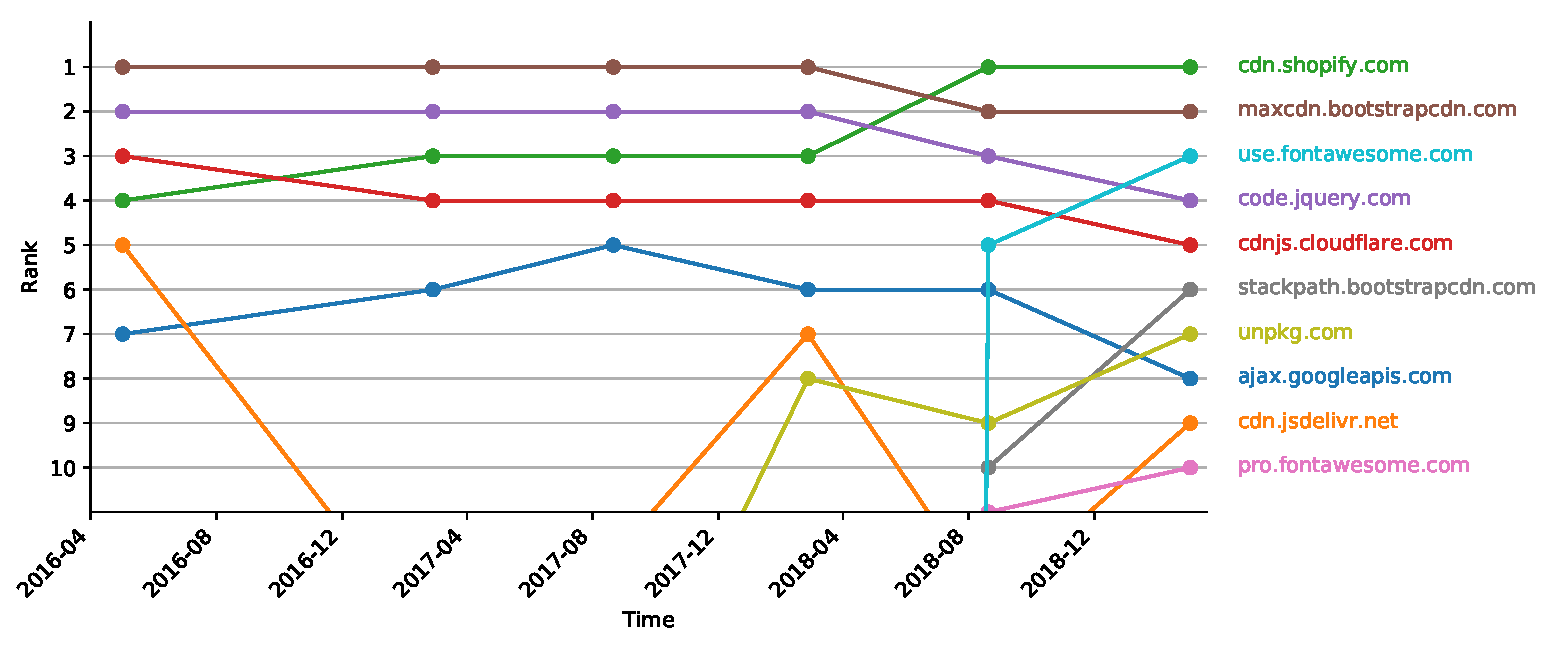
\includegraphics[width=1.6\columnwidth]{../../notebooks/08_topk_evolution}
	\caption{PDF/CDF of the top 20 domain names targeted by tags (script or link) that specifies the integrity attribute}
	\label{fig:08}
\end{figure*}

\begin{figure}[h]
	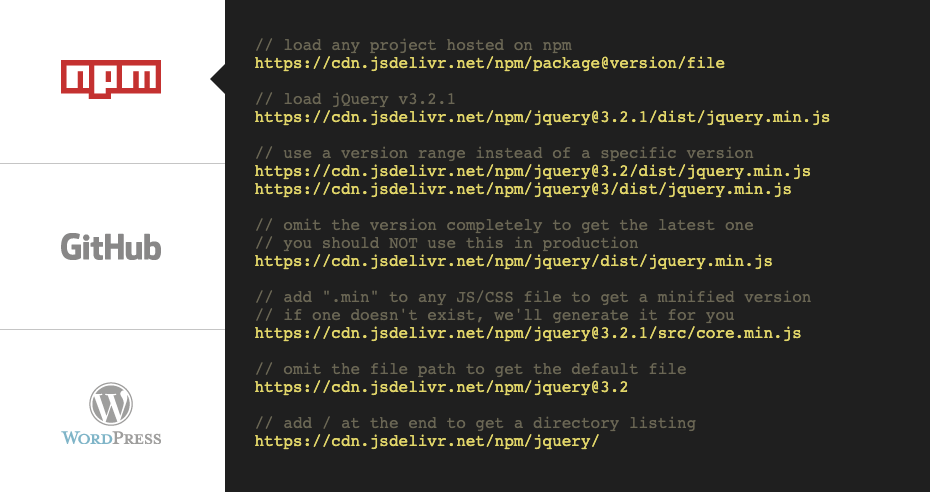
\includegraphics[width=\columnwidth]{figures/jsdelivr}
	\caption{jsDelivr relax integrity to gracefully upgrade subresources}
	\label{fig:jsdelivr}
\end{figure}


%\begin{figure}[h]
%	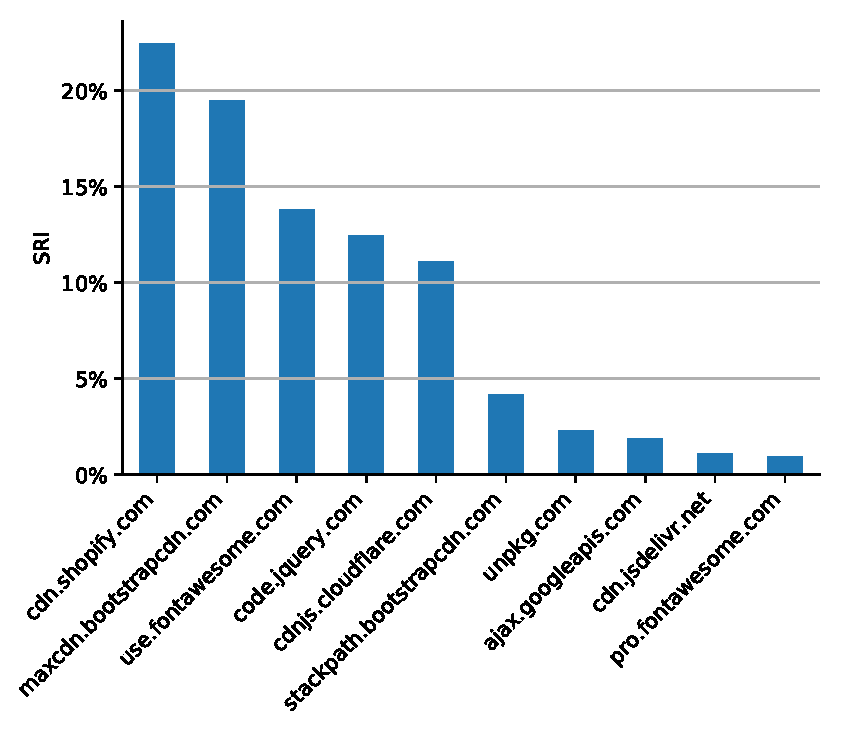
\includegraphics[width=\columnwidth]{../../notebooks/08_topk_sri_domain}
%	\caption{PDF/CDF of the top 10 domain names targeted by tags (script or link) that specifies the integrity attribute}
%	\label{fig:08}
%\end{figure}


\subsubsection{Use of the require-sri-for directive}

The \textit{require-sri-for} directive leverage the ability to ensure that all subresources of a webpage specify the integrity attribute.
As a result, it allows an elegant separation of concerns between system administrators and web developers.
We queried the \CCSnapshotLatest snapshot of the \CCSRI dataset to obtain the percentage of webpages that specify the \textit{require-sri-for} directive in their HTTP headers.
In practice, only a marginal number of webpages (\CCRequireSriForP) use this directive.
Given this poor adoption, its upcoming deprecation by Web browsers is clearly justified.



\section{Browser Support} \label{sec:browser-support}

\subsection{Methodology}

We created a testbed consisting in webpages to check the implementation of the SRI recommendation in major browsers.
We visited these webpages with major browsers (Chrome, Mozilla Firefox, Safari, Edge, Explorer, Opera) to collect data.

\subsection{Tests}

Table~\ref{tbl:browser-support} summarizes the tests we executed in different browsers.
Hereafter, we provide implementation details that allow to reproduce these tests.

\subsubsection{Support require-sri-for}
We tested if browsers enforce the require-sri-for directive that can be specified through HTTP headers.
Overall, we noticed that this directive is not supported in web browsers.
In Chrome and Firefox it has to be explicitly turned on with a flag when launching the browser.
In addition, its removal from the W3C recommendation is scheduled.

\subsubsection{Support well formed sha2 checksums}
We tested if browsers support the algorithms from the sha2 family (sha256, sha384 and sha512) and noticed that they behave according to the recommendation.

\subsubsection{Support empty integrity attribute}
We tested if browsers should include the subresources with an empty integrity attribute and noticed that they behave according to the recommendation.

\subsubsection{Support missing base64 trailing equals}
We tested if the removal of trailing equals (=) introduced by the encoding of the checksum in base64 affects the inclusion of the subresources.
We found that all browsers support the removal of these extra characters.

\subsubsection{Support conflicting checksums}
We tested if browsers support conflicting checksums, i.e., what happen if two different sha256 checksums are specified for the same target.
We found that all browsers support this feature and execute the script if one of the two checksums matches.

\begin{lstlisting}[language=HTML, basicstyle=\small]
<script src="http://.../script.js" 
	integrity="sha256-v1... sha256-v2..." 
	crossorigin="anonymous"></script>
\end{lstlisting}

\subsubsection{Block well formed wrong checksum}
We tested if browsers prevent the execution of a script that specifies the wrong integrity attribute.
We found that all browsers behave consistently.

\begin{lstlisting}[language=HTML, basicstyle=\small]
<script src="http://.../script.js" 
	integrity="sha256-wrong..." 
	crossorigin="anonymous"></script>
\end{lstlisting}

\subsubsection{Block malformed checksum}
We tested if browsers prevent the execution of malformed integrity attributes, e.g., by using the string "malformed" as a value for the integrity attribute.
Surprisingly, an error was raised by most browser, but the execution of the script was not prevented.

\begin{lstlisting}[language=HTML, basicstyle=\small]
<script src="http://.../script.js" 
	integrity="malformed" 
	crossorigin="anonymous"></script>
\end{lstlisting}

\subsubsection{Block md5 checksum}
Knowing from our analysis that some websites specify md5 checksums, we specified one to check if such inclusion is prevented.
Interestingly, we observed errors similar to the one raised for malformed checksums.
In other words, the integrity attribute is considered as malformed, hence the script is executed.

\begin{lstlisting}[language=HTML, basicstyle=\small]
<script src="http://.../script.js" 
	integrity="md5-MGI0NTUx..." 
	crossorigin="anonymous"></script>
\end{lstlisting}

\subsubsection{Block missing hash prefix}
Similarly, knowing that some web developers forget the dash between the algorithm and the digest, we tested this corner case and noticed that the scripts get executed.

\begin{lstlisting}[language=HTML, basicstyle=\small]
<script src="http://.../script.js" 
	integrity="sha256ivzZrYOz..." 
	crossorigin="anonymous"></script>
\end{lstlisting}

\subsection{Results}

\begin{table*}[h]
\rowcolors{3}{white}{tblgray}
\begin{tabular}{l|cccccc|cccc|c}
\toprule
% Platform
& \multicolumn{6}{c|}{\faDesktop} 
& \multicolumn{4}{c|}{\faMobile} 
& \\
% Browser
& \mlc{\faChrome \\ \footnotesize{Chrome}} 
& \mlc{\faFirefox \\ \footnotesize{Firefox}}
& \mlc{\faSafari \\ \footnotesize{Safari}} 
& \mlc{\faEdge \\ \footnotesize{Edge}}
& \mlc{\faEdge \\ \footnotesize{Explorer}}
& \mlc{\faOpera \\ \footnotesize{Opera}}
& \mlc{\faAndroid \\ \footnotesize{Android}}
& \mlc{\faChrome \\ \footnotesize{Chrome}} 
& \mlc{\faFirefox \\ \footnotesize{Firefox}}
& \mlc{\faSafari \\ \footnotesize{Safari}}
& \mlc{\faWWWC \\ \footnotesize{Spec.}}\\	
\bottomrule	
\textit{Support require-sri-for}					& \yessymbol* &	\yessymbol*	& \nasymbol & \nasymbol & \nasymbol & \nasymbol & \nasymbol & \nasymbol & \nasymbol & \nasymbol & \yessymbol* \\
\textit{Support well formed sha2 checksums}				& \yessymbol & \yessymbol & \yessymbol & \nasymbol & \nasymbol & \yessymbol & \nasymbol & \yessymbol & \yessymbol & \yessymbol & \yessymbol \\
\textit{Support empty integrity attribute}		& \yessymbol & \yessymbol & \yessymbol & \nasymbol & \nasymbol & \yessymbol & \nasymbol & \yessymbol & \yessymbol & \yessymbol & \yessymbol \\
\textit{Support missing base64 trailing equals}	& \yessymbol & \yessymbol & \yessymbol & \nasymbol & \nasymbol & \yessymbol & \nasymbol & \yessymbol & \yessymbol & \yessymbol & \yessymbol \\
\textit{Support conflicting checksums}			& \yessymbol & \yessymbol & \yessymbol & \nasymbol & \nasymbol & \yessymbol & \nasymbol & \yessymbol & \yessymbol & \yessymbol & \yessymbol \\
\textit{Block well formed wrong checksum}					& \yessymbol & \yessymbol & \yessymbol & \nasymbol & \nasymbol & \yessymbol & \nasymbol & \yessymbol & \yessymbol & \yessymbol & \yessymbol \\
\textit{Block malformed checksum	}				& \nosymbol & \nosymbol & \nosymbol & \nasymbol & \nasymbol & \nosymbol & \nasymbol & \nosymbol & \nosymbol & \nosymbol & \nasymbol \\
\textit{Block md5 checksum}						& \nosymbol & \nosymbol & \nosymbol & \nasymbol & \nasymbol & \nosymbol & \nasymbol & \nosymbol & \nosymbol & \nosymbol & \nasymbol \\
\textit{Block missing hash prefix}				& \nosymbol & \nosymbol & \nosymbol & \nasymbol & \nasymbol & \nosymbol & \nasymbol & \nosymbol & \nosymbol & \nosymbol & \nasymbol \\
\bottomrule
\end{tabular}
\caption{Browser behaviors and recommended implementation regarding subresource handling. (\textit{*A flag activates require-sri-for in Chrome and Firefox and the removal of the directive from the W3C recommendation is scheduled}).}
\label{tbl:browser-support}
\end{table*}

\section{Web Developer Experience}

We interview web developers and system administrators to assess their understanding of the SRI recommendation.

\subsection{Screening Questionnaire}

Research questions (Draft):

\begin{enumerate}
	\item Age/Gender/Profession/Education/...
	\item Are you a web developer? If yes, since...
	\item Are you a system administrator? If yes, since...
	\item ...
\end{enumerate}


\subsection{Interview protocol}

Research questions (Draft):

\begin{enumerate}
	\item Have you already heard about SRI?
	\item Have you already used SRI?
	\item Have you already encountered the integrity attribute in a web page?
	\item If so, in which HTML element have you encountered this attribute?
	\item What is the purpose of the integrity attribute?
	\item Among these values for the integrity attribute, which one are well formed?
	\item Can SRI be used in place of HTTPS? Why?
	\item Can HTTPS be used in place of SRI? Why?
	\item Have you already integrated a third party library on a website?
	\item If so, how did you do?
	\item If so, what were your security concerns in doing so?
	\item Would you use SRI with other kind of subresources?
	\item ...
\end{enumerate}





\section{Adoption incentives} \label{sec:discussion}

\subsection{Methodology}

To understand what could be done to improve the adoption of SRI, we compute the list of the most popular javascript and css subresources with or without the integrity attribute in a \num{1}\% random sample of the February 2019 \CC dataset.
For every subresource present in this sample, we take the one with an absolute url that ends with the \textit{*.js} or \textit{*.css} extensions.

\subsection{Results}

Table~\ref{table:top-libraries} shows some discrepancy between subresources with and without the integrity attribute.
In other words, there is plenty of room left to improve the adoption of SRI.
Here, we can categorize 


\begin{enumerate}
	\item 
		The results falling in the add-on category can hardly adopt SRI.
		For instance, as the social buttons and tracking codes from major providers are constantly evolving, the coupling introduced by the integrity attribute is unbearable.
		However, this question the responsibility of web developers when integrating such third-party libraries.
	\item
		The snippet provided by Facebook loads the script asynchronously which explains why their add-on is not included in the results.
\end{enumerate}


\begin{table*}[h]
\rowcolors{1}{white}{tblgray}
\begin{tabular}{ccccccc}
\toprule
\textbf{Rank} & \textbf{Perc.}	& \textbf{Name}       & \textbf{Type} & \textbf{Snippet}	& \textbf{SRI}	& \textbf{Adoption} \\ 
\bottomrule
1             & \num{11.72}\%	& Google Syndication  & Add-on        & \yessymbol			&				&                   \\
2             & \num{6.39}\%		& jQuery              & Library       & \yessymbol			& \yessymbol	& Mar.16            \\
3             & \num{5.04}\%		& Wordpress           & Platform      & 						&				&                   \\
4             & \num{2.62}\%		& Google APIs         & Add-on        & \yessymbol			&				&                   \\
5             & \num{2.40}\%		& Blogger             & Platform      & 						& 				&                   \\
6             & \num{2.21}\%		& FontAwesome         & Library       & \yessymbol			& \yessymbol	& N/A				\\
7             & \num{1.41}\% 	& TripAdvisor CDN	  & Platform      & 						&				&                   \\
8             & \num{1.38}\%		& Twitter             & Add-on        & \yessymbol			&				&                   \\
9             & \num{1.29}\%		& SmugMug             & Platform      &						&				&                   \\
10            & \num{1.21}\%		& Squarespace         & Platform      & 						&				&                   \\
11            & \num{1.21}\%		& Bootstrap           & Library       & \yessymbol			& \yessymbol	& Oct.15            \\
12            & \num{1.19}\%		& WIX                 & Platform      &						&				&                   \\
13            & \num{1.13}\%		& Google Ad Services  & Add-on        & \yessymbol			&				&                   \\
14            & \num{0.94}\%		& Google Tag Services & Add-on        & \yessymbol			&				&                   \\
15            & \num{0.94}\%		& jQueryUI            & Library       & \yessymbol			& \yessymbol	& Mar.16            \\
16            & \num{0.87}\%		& Google Recaptcha    & Add-on        & \yessymbol			& 				&                   \\
17            & \num{0.86}\%		& Google Analytics    & Add-on        & \yessymbol			&				&                   \\
18            & \num{0.73}\%		& BigCommerce         & Platform      &						& 				&                   \\
19            & \num{0.73}\%		& Shopify             & Platform      &						& \yessymbol	&                   \\
20            & \num{0.66}\%		& CookieConsent2      & Library       & \yessymbol			&				&                   \\ 
\bottomrule	
\end{tabular}
\caption{Most popular third-party resources referenced among script and link elements (N=\num{158284348})}
	\label{table:top-libraries}
\end{table*}




\section{Related Work} \label{sec:rw}

SRI~\cite{w3c_subresource_2016,shah_measurement_2018,shah_securing_2017,van_acker_measuring_2017,anis_securing_2018}.

SRI limitations for unknown content~\cite{kumar_security_2017,soni_sicilian_2015}.

Download checksums~\cite{cherubini_towards_2018}.

Third-party libraries~\cite{lauinger_thou_2017}.

Security awareness assessement~\cite{krombholz_if_2019}.

Content security policy~\cite{calzavara_content_2016,afanasyev_content-based_2016,van_acker_measuring_2017,some_content_2017}.

Alternatives to SRI~\cite{matulevicius_ensuring_2018,calzavara_content_2016,kumar_security_2017,salvador_wraudit_2018}.

Risks and Motivations~\cite{bodden_control_2017,romagna_hacktivism_2017,kerschbaumer_enforcing_2016,lavrenovs_http_2018,arshad_large-scale_2018,eden_major_2018,van_acker_measuring_2017}.

\begin{itemize}
	\item Checksums and integrity verification
	\item subresource integrity (SRI)	
\end{itemize}


\section{Conclusion} \label{sec:conclusion}

\begin{acks}
The authors express their sincere gratitude to the anonymous reviewers for their insightful feedback. The authors also warmly thank Holly Cogliati for her great editing job on the manuscript and Romain Artru for his help in the implementation of the analysis scripts. The work was partially funded with grant \#19024 from the Hasler Foundation and  a UNIL-HEC Lausanne Research Fund.
\end{acks}

%\immediate\write18{./fetchbib.sh}
\balance
\bibliographystyle{ACM-Reference-Format}
\bibliography{main.bib}

% TODO: item vs. inlineitem, circles vs. letters
\appendix

\end{document}
